
\documentclass[12pt]{article}

\usepackage{fancyhdr}
\usepackage{lipsum}
\usepackage{lastpage}
\usepackage{titleref}
\usepackage[ngerman]{babel}
\usepackage{datetime}
\usepackage{makecell}
\usepackage{pdfpages}

\newdateformat{deformat}{\THEDAY.\THEMONTH.\THEYEAR}

\makeatletter
\newcommand*{\currentname}{\TR@currentTitle}
\makeatother

% Turn on fany style
\pagestyle{fancy}
% Clear the header and footer
\fancyhead{}
\fancyfoot{}

\begin{document}

\begin{center}
\begin{tabular}{ |c|c|c| }

\hline
Nachname & Vorname & Matrikelnummer \\
\hline
\makecell{ 1. Bartussek } & Dario & 2072140 \\
\hline
\makecell{ 2. Lukic } & Ivan & 2067465 \\
\hline
\makecell{ 3. Fakher Aldein } & Majdi & 2070203 \\
\hline

\end{tabular}
\end{center}

Für Quellen siehe https://github.com/dbartussek/SEProjekt

\newpage
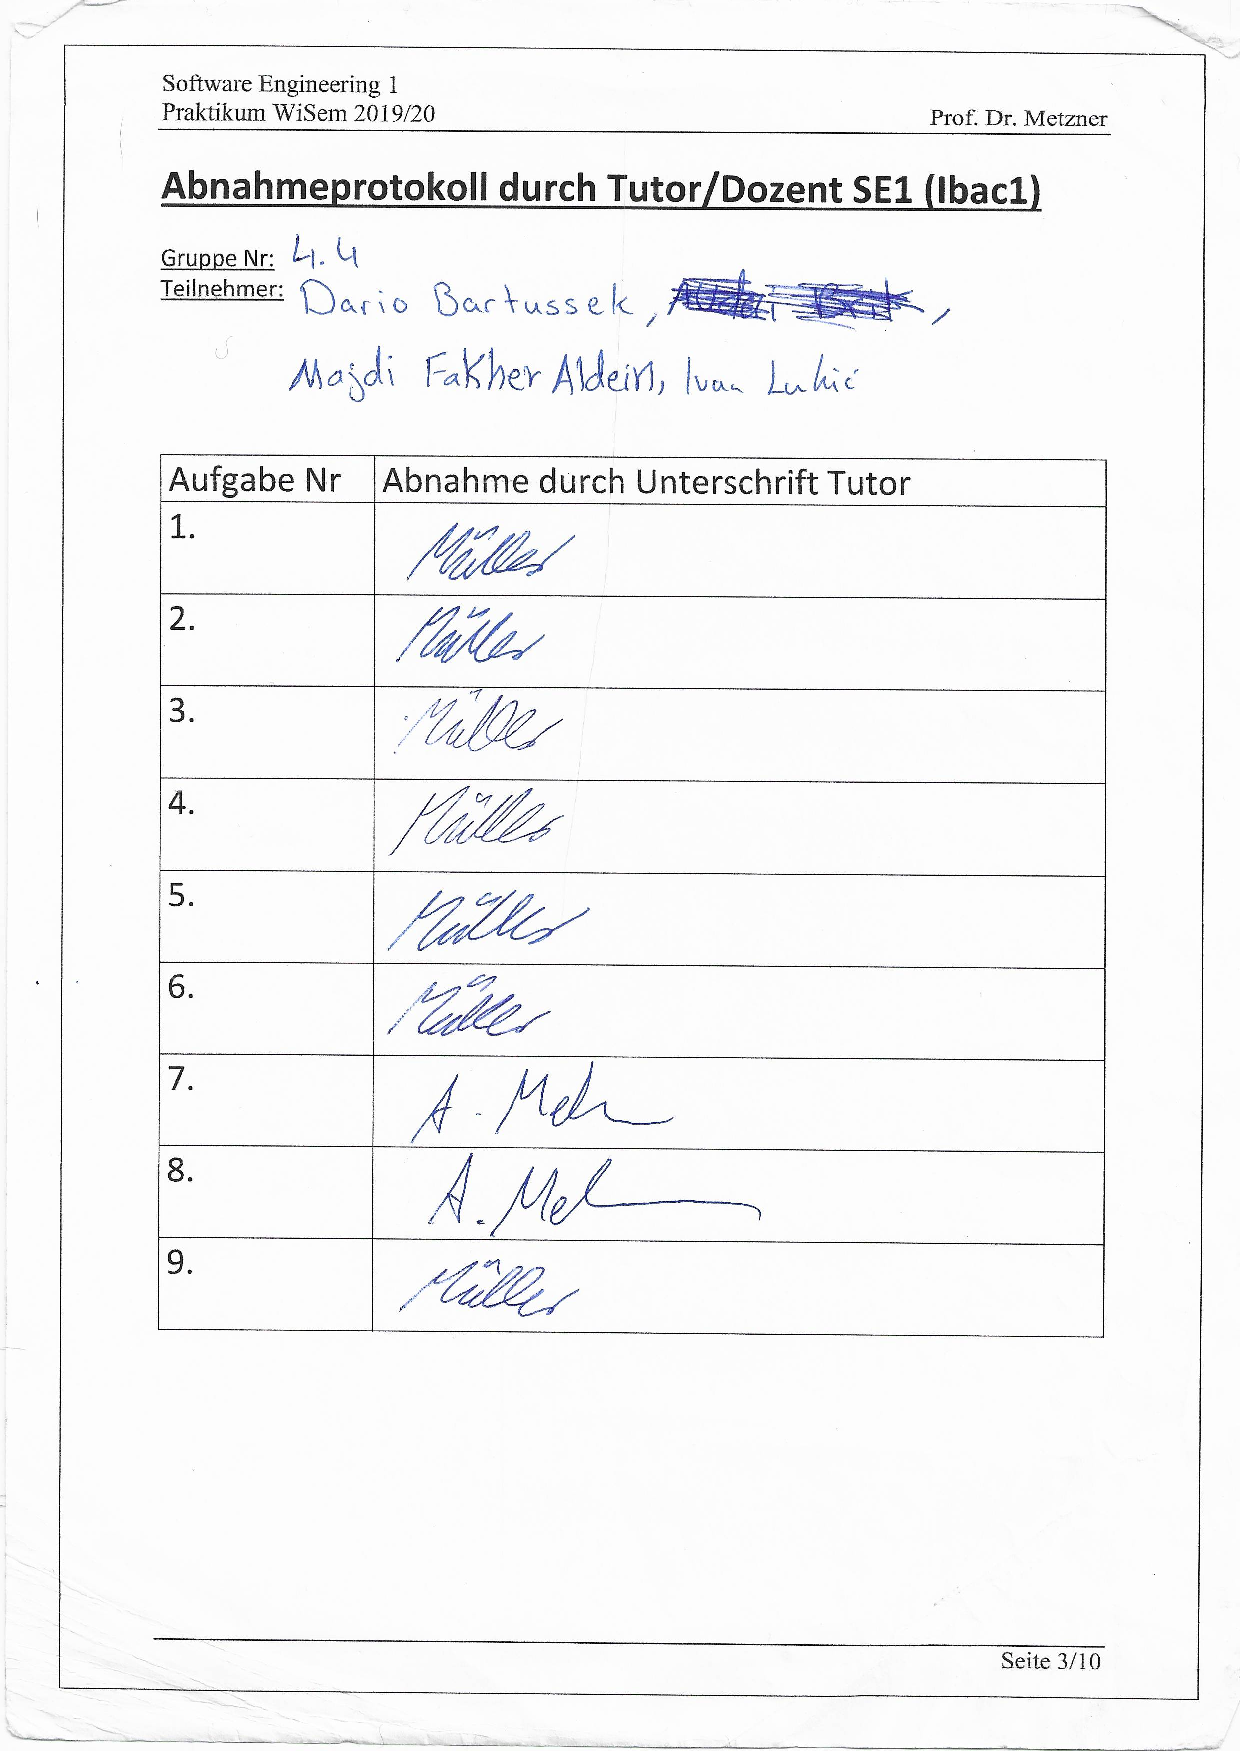
\includepdf[pages=-]{unterschriften.pdf}

\newpage
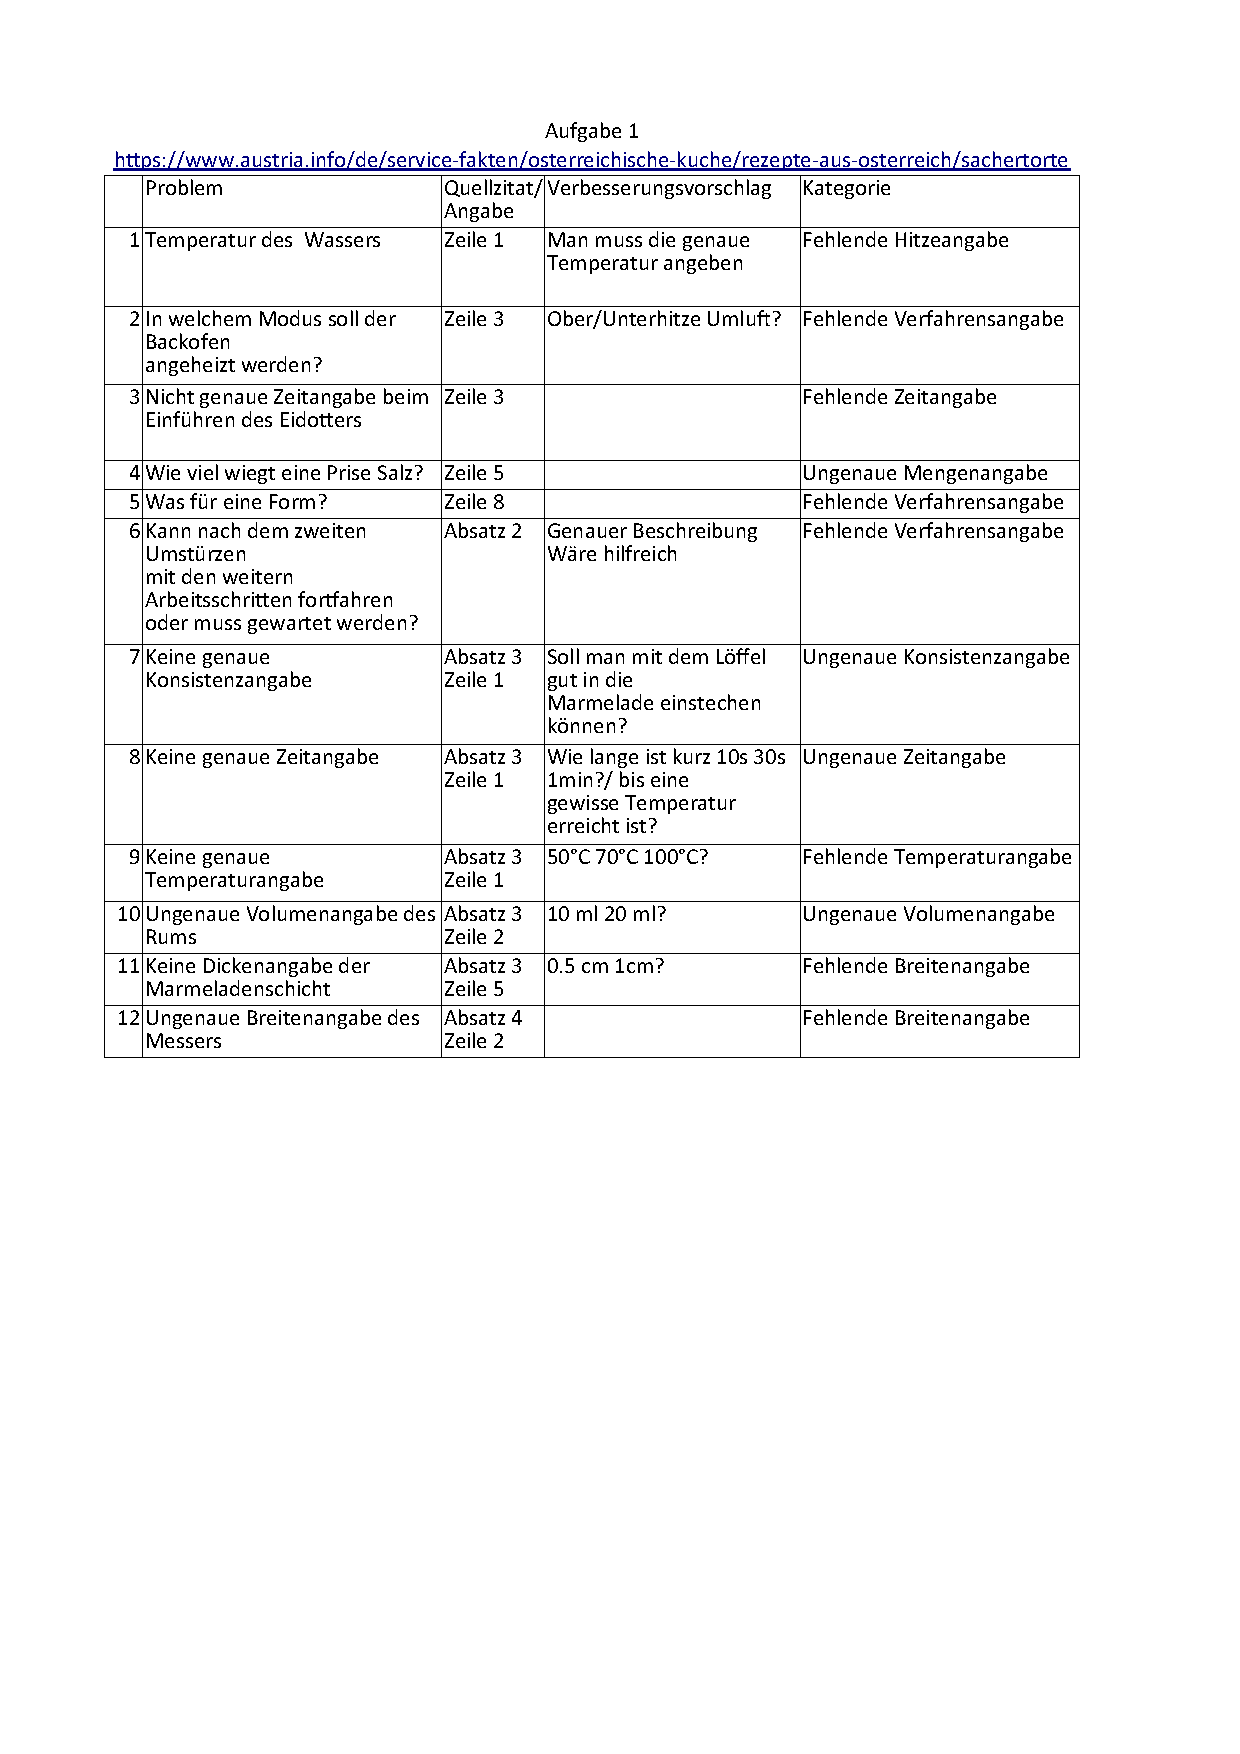
\includepdf[pages=-]{aufgabe1.pdf}

\newpage
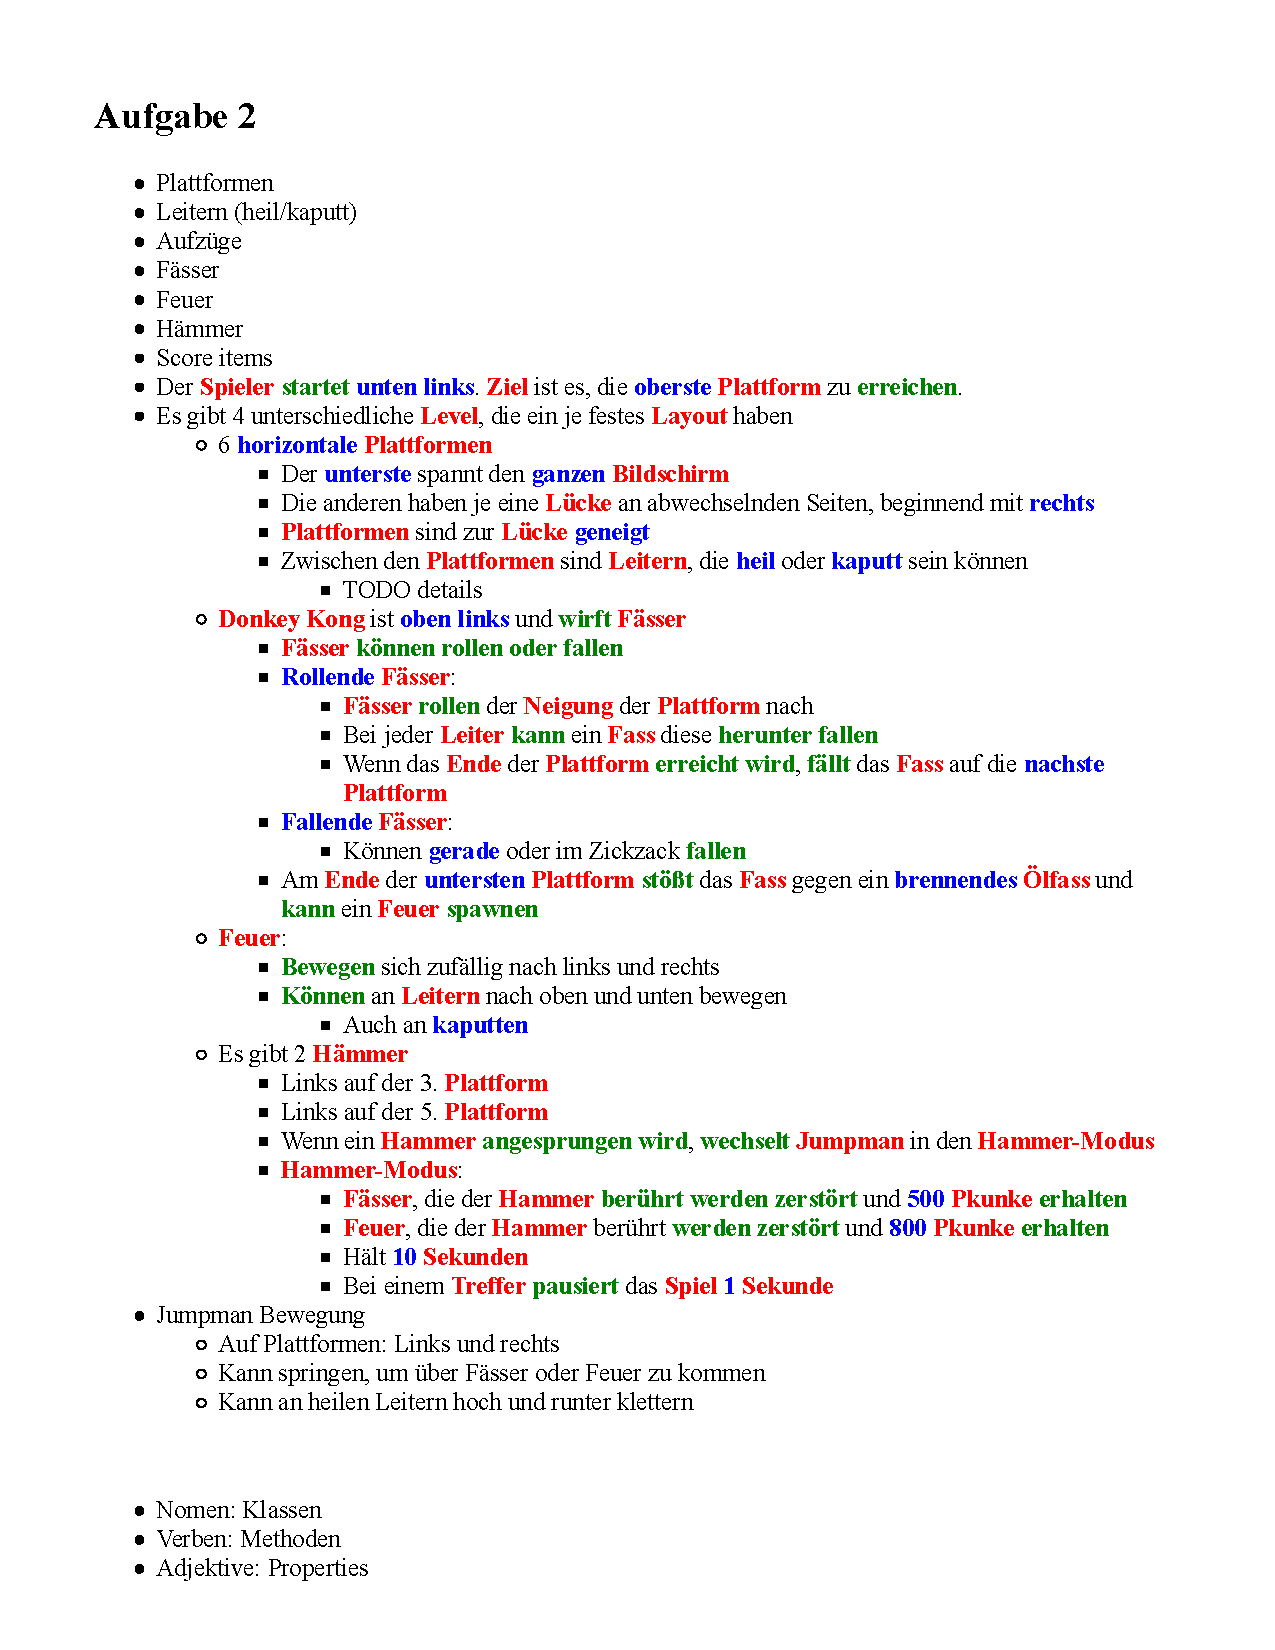
\includepdf[pages=-]{aufgabe2.pdf}

\newpage
\includepdf[pages=-]{aufgabe3/Pflichtenheft.pdf}

\newpage

\includepdf[pages=2]{aufgabe4.pdf}

\newpage
\includepdf[pages=-]{aufgabe5.pdf}

\newpage
\includepdf[pages=-]{aufgabe6a.pdf}

\newpage
\includepdf[pages=-]{aufgabe6b.pdf}

\newpage
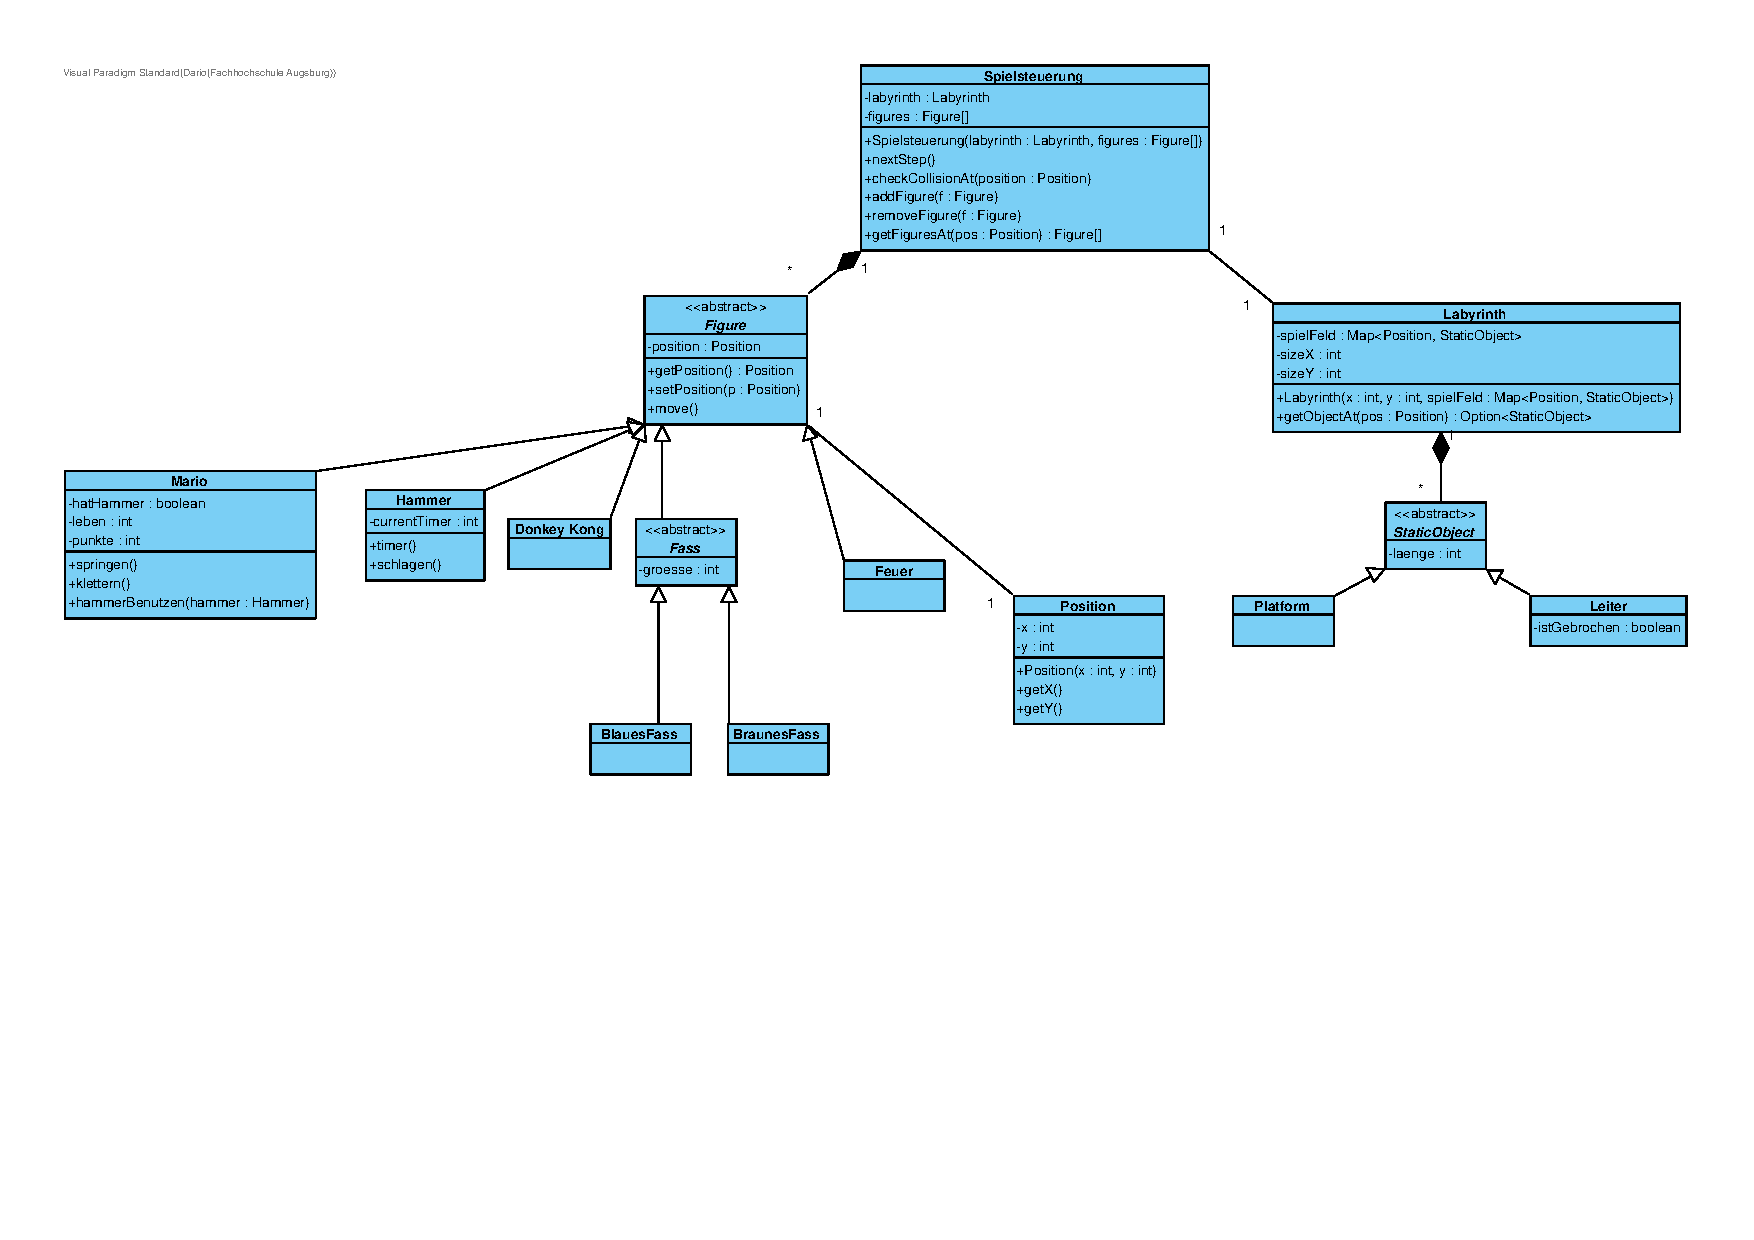
\includepdf[pages=-]{aufgabe7.pdf}

\newpage
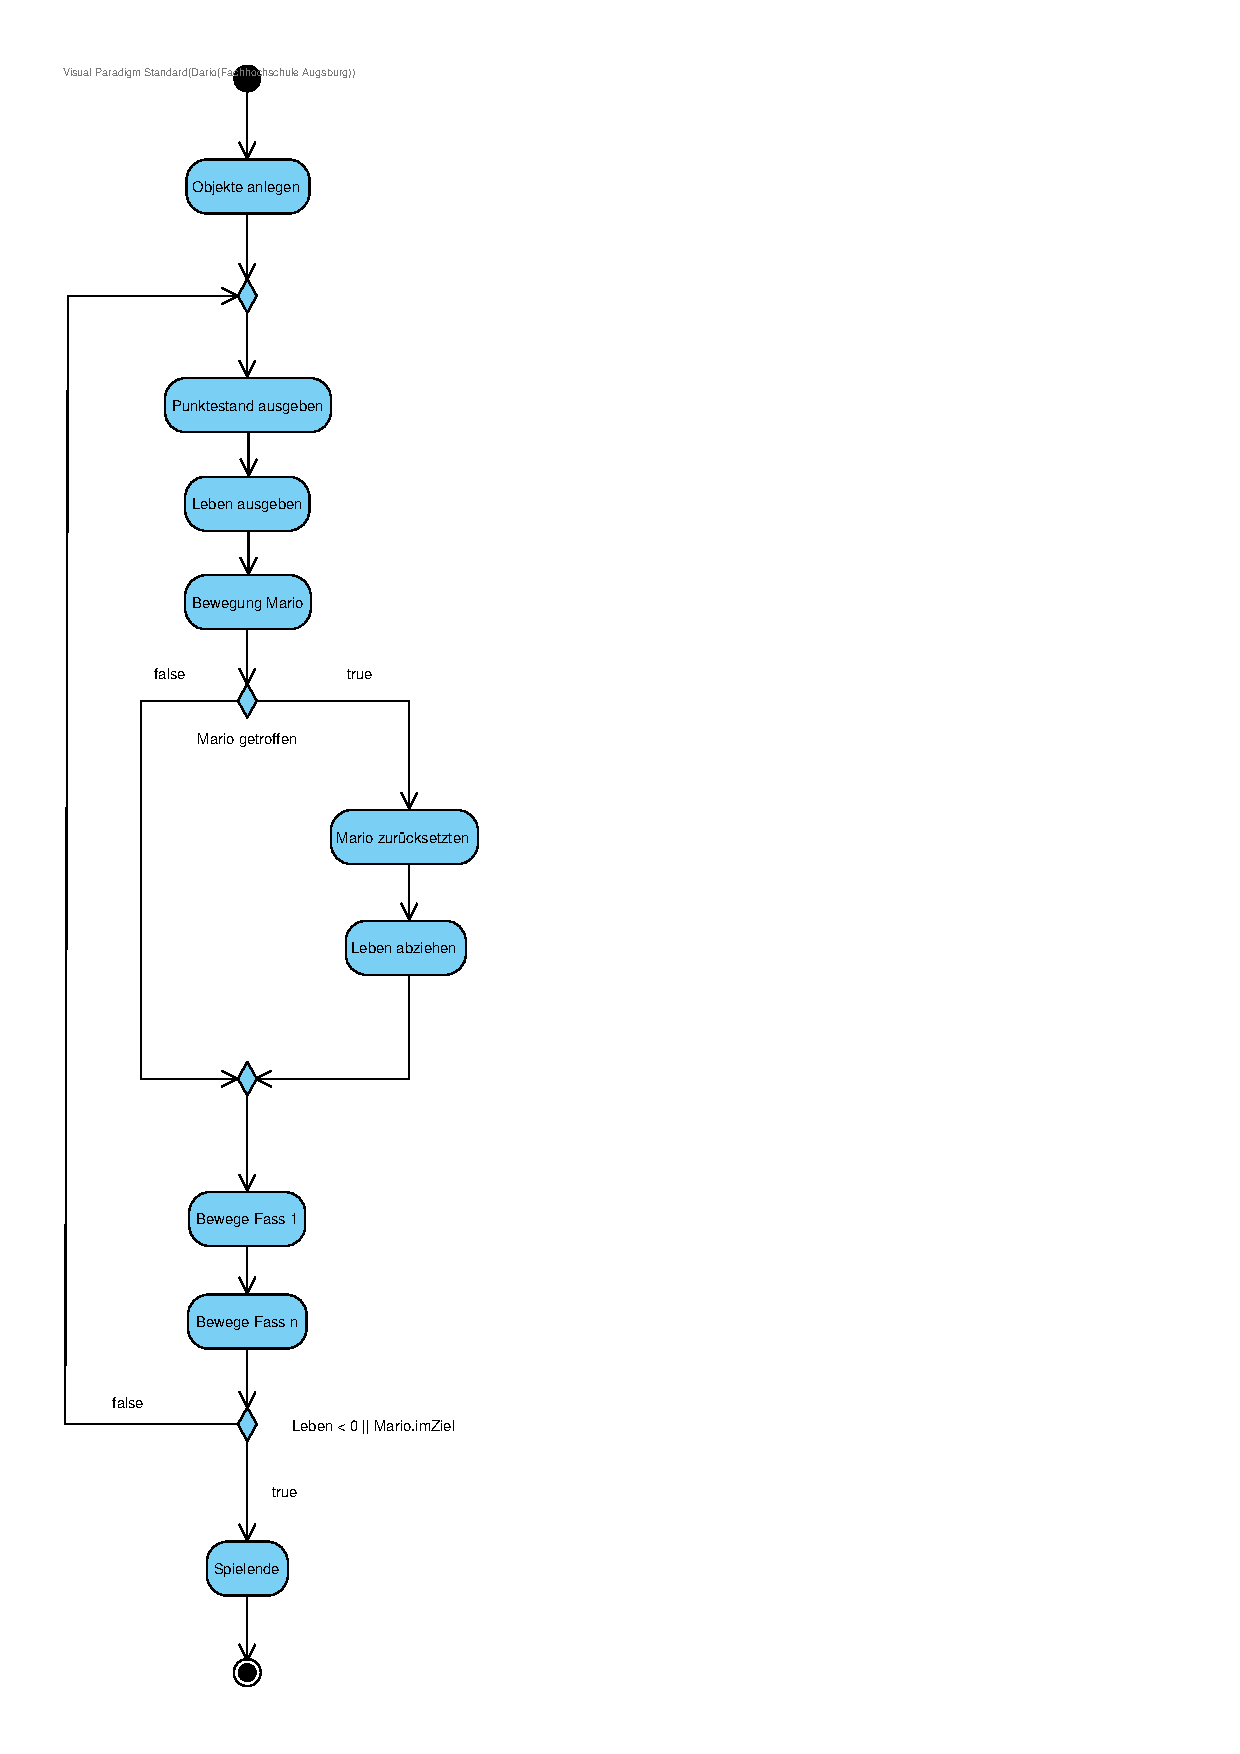
\includepdf[pages=-]{aufgabe8a.pdf}

\newpage
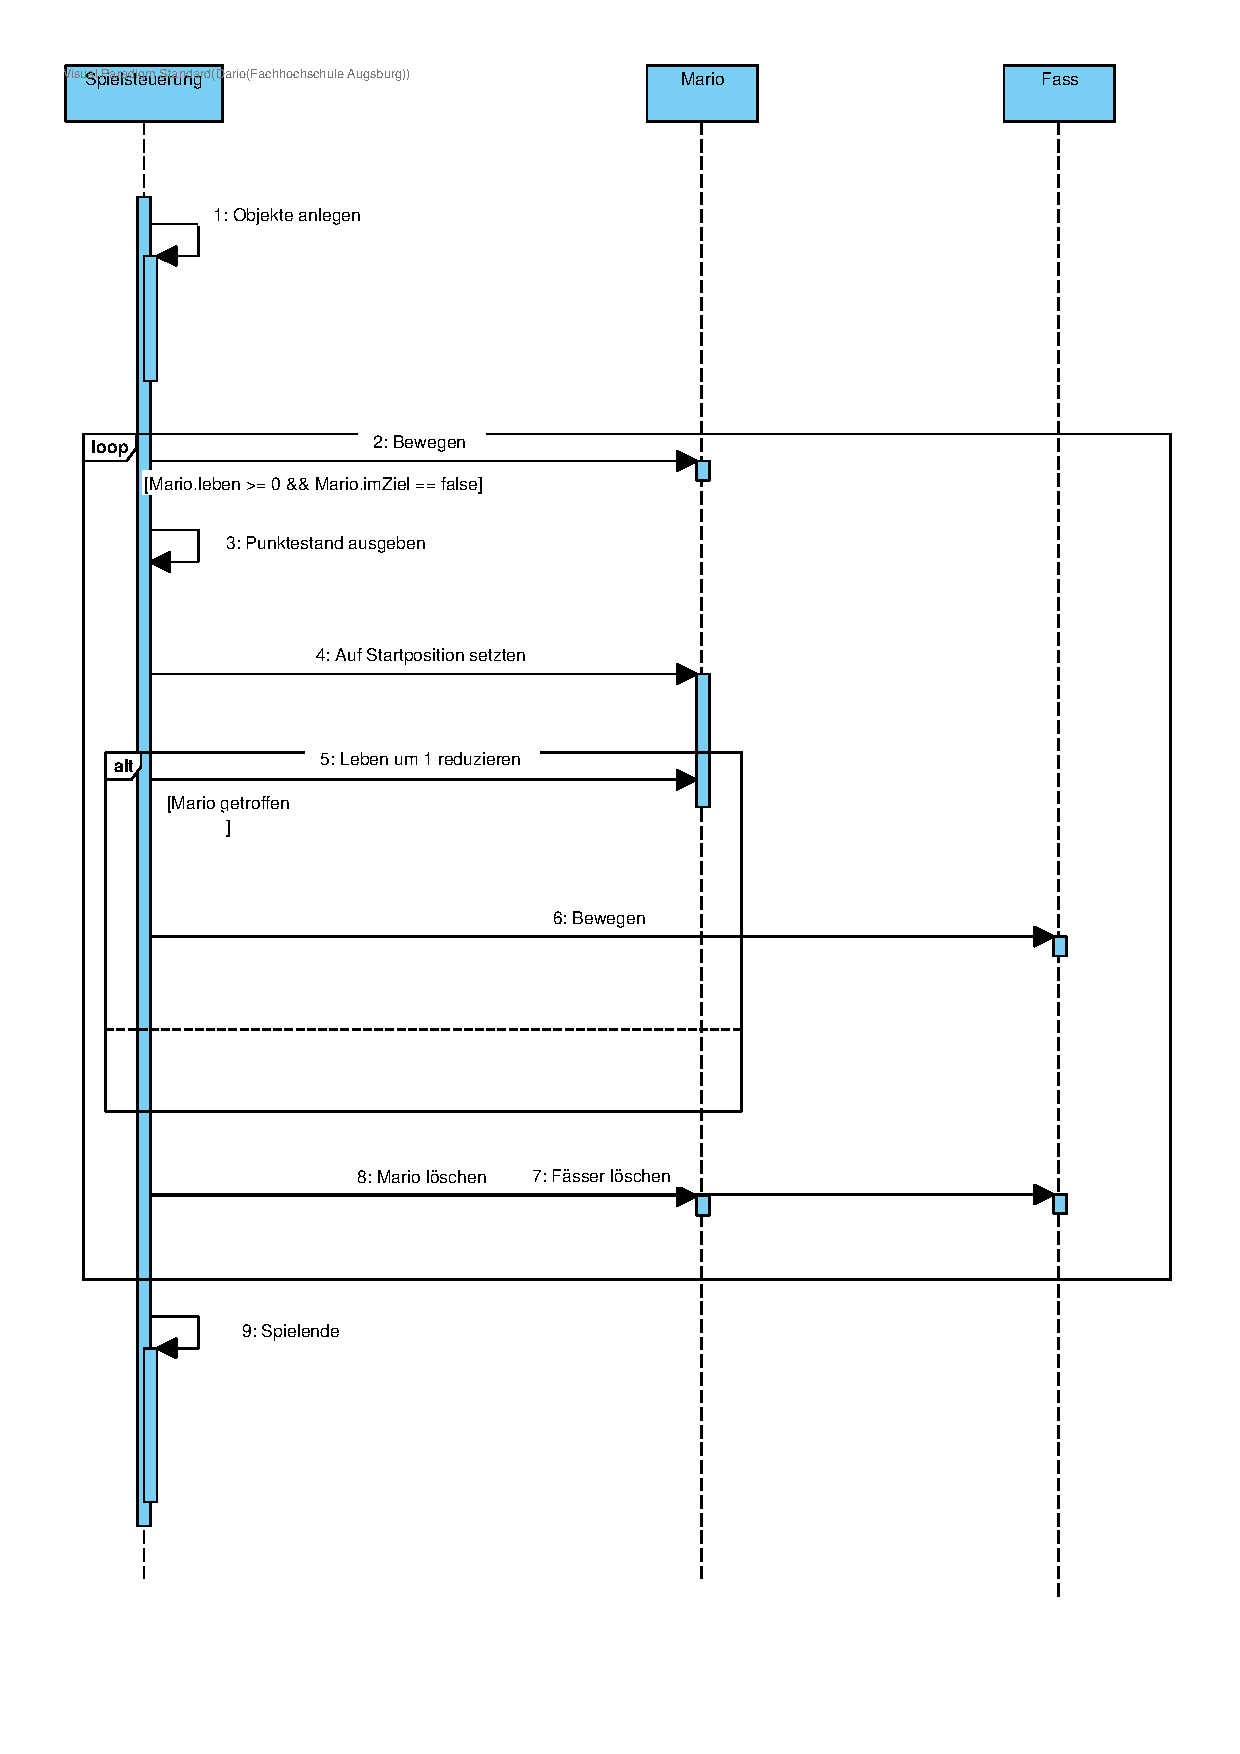
\includepdf[pages=-]{aufgabe8b.pdf}

\newpage
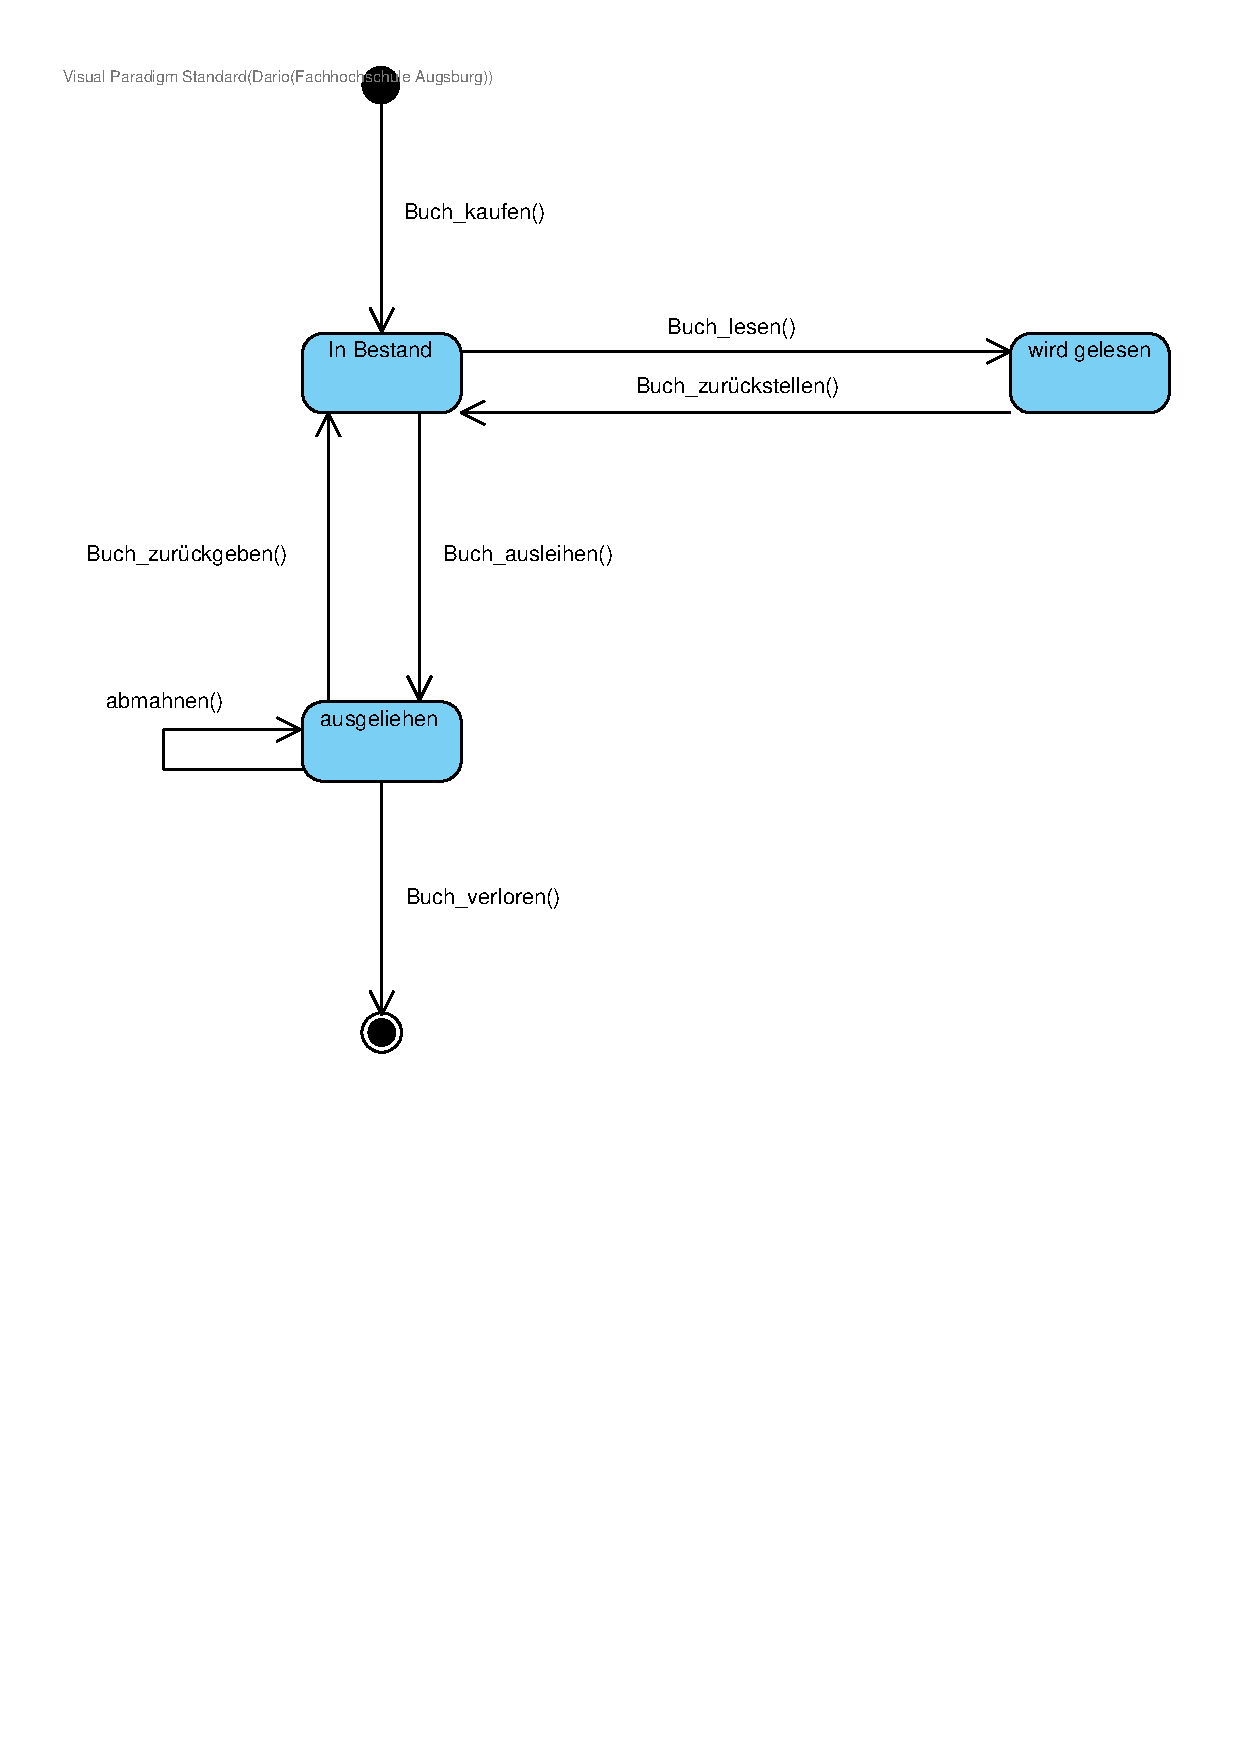
\includepdf[pages=-]{aufgabe9.pdf}

\end{document}
